\documentclass[12pt]{beamer}
\usetheme{Boadilla}

\usepackage[utf8]{inputenc}
\usepackage{graphicx}
\usepackage{amsmath}
\usepackage{tikz}
\usetikzlibrary{shapes.geometric}
\usetikzlibrary{arrows.meta,arrows}
\usetikzlibrary{intersections}
\setbeamersize{text margin left=10mm,text margin right=10mm}

\title{Numerical Methods for Finance}
\subtitle{Second Order Discretization Schemes for CIR Processes}
\author{Espel, Groeneweg, Pavon, Tomas}
\institute{Imperial College London}
\date{\today}

\begin{document}

\begin{frame}
    \titlepage
\end{frame}


\begin{frame}
\frametitle{Outline}
\tableofcontents
\end{frame}

\begin{frame}
\frametitle{Introduction}
\begin{itemize}
  \item CIR schemes are frequently used.
  \item However, usual numerical schemes can fail when one tries to simulate them.
  \item We have implemented a solution proposed in 2008 by Aurélien Alfonsi in his paper \textit{High order discretization schemes for the CIR process: application to A ne Term Structure and Heston models} (hal-00143723).
  \item We have calibrated and simulated some results with the Heston model.
\end{itemize}
\end{frame}


\section{Discretizing CIR Processes}
\frame{\tableofcontents[currentsection]}

\begin{frame}
\frametitle{CIR Processes}
Noting $X^{x}_{t}$ the solution of the CIR (Cox-Ingersoll-Ross) SDE:
\begin{align*}
dX^{x}_{t} & = a - kX^{x}_{t} + \sigma \sqrt{X^{x}_{t}} dW_{t} \\
X^{x}_{0} & = x, x \in \mathbb{R_{+}}
\end{align*}
\begin{itemize}
  \item The main difficulty is to disctrize the process around 0, where since the square root is not Lipschitzian.
  \item Euler and Milstein schemes are usually not well defined, and generate negative values.
  \item Aurélien Alfonsi presents very efficient schemes for general affine diffusions, without any restriction on the parameters.
\end{itemize}
\end{frame}


\begin{frame}
\frametitle{CIR Processes - Why it matters}
Noting $X^{x}_{t}$ the solution of the CIR (Cox-Ingersoll-Ross) SDE:
\begin{align*}
dX^{x}_{t} & = a - kX^{x}_{t} + \sigma \sqrt{X^{x}_{t}} dW_{t} \\
X^{x}_{0} & = x, x \in \mathbb{R_{+}}
\end{align*}
Large values of $\sigma$:
\begin{itemize}
  \item No problem when the CIR process represents the short interest rate.
  \item Issues when the CIR process respresents default intensity in credit risk or the stock volatility like in the Heston model.
\end{itemize}
\end{frame}

\begin{frame}
\frametitle{How usual numerical schemes can fail}
Qualitative analysis: when $X$ is very close to $0$, then the SDE becomes approximately

$$
dX^{x}_{t} \approx a + \sigma \sqrt{X^{x}_{t}} dW_{t}
$$

There are two possible regimes:
\begin{itemize}
	\item If $\sigma << a$: $X$ will mostly stay positive
	\item If $\sigma >> a$: $X$ may become negative!
\end{itemize}
\end{frame}

\begin{frame}
\frametitle{How usual numerical schemes can fail}
 \begin{tikzpicture}

 % Line for current point of the scheme
 \draw [->] (0,-3) -- (0,3);
 \node [below, black] at (0,-4) {$t$};

 % Draw transition between the two times
 \draw [->] (1,1) -- (4,1);
 \node at (2.5,1.5) {$ p^{X^{x}_{t}}_{t} $, transition density};

 % Current point
 \draw[-] [draw=black, very thick] (-0.1,0.5) --  (0.1,0.5);
 \node [below left,black] at (0,0.5) {$X^{x}_{t}$};

 % Line for next possible points
 \draw[->] (5,-3) -- (5,3);
 \node [below, black] at (5,-4) {$t + \Delta t$};

 % Distributions depending on regime
 % sigma_high = 4.0, a_high = 1.0
 % sigma_low = 1.0, a_low = 1.0

 % distribution for high
 \draw [red, domain=-3:0, variable = \y] plot ({5.0 + exp( -  (\y  -1)*(\y  -1) /(2.0 * 16.0))},{\y});
 \draw [red, domain=-3:0, variable = \y] plot ({5.0 + exp( -   (\y  -1)*(\y  -1) /(2.0 * 1.0))},{\y});

 % distribution for low
 \draw [green, domain=0:3, variable = \y] plot ({5.0 + exp( -  (\y  -1)*(\y  -1) /(2.0 * 16.0))},{\y});
 \draw [green, domain=0:3, variable = \y] plot ({5.0 + exp( -  (\y  -1)*(\y  -1) /(2.0 * 1.0))},{\y});

 % Line we should not cross
 \node [below left, black] at (0,0) {0};
 \draw[dashed] [red] (0,0) -- (7,0);
 \node [below, black] at (8,-3) {Negative values of $X^{x}_{t+\Delta t}$ } ;
 \node [below, black] at (8,3) {Positive values of $X^{x}_{t+\Delta t}$};

 \end{tikzpicture}


\end{frame}

\begin{frame}
\frametitle{Regime $\sigma << a$ ( $\dfrac{\sigma^{2}}{4} \leq a $) }

How do we keep the process positive and the scheme precise? \\

Replace the original distribution by another with compact support. The higher the degree of precision, the more this variables has to account for the tail behaviour of the subsituted one. \\

Alfonsi shows that we keep the scheme of order $\nu$, if we subsitute the random variable with one that matches the first $2\nu +1$ moments.

Using discrete random variables, we can control the tail probability and ensure the process stays positive.
\end{frame}

\begin{frame}
\frametitle{Regime $\sigma >> a$ ( $\dfrac{\sigma^{2}}{4} > a $) }

Alonfsi proves:

\begin{itemize}
	\item When $X^{x}_{t}$ is far away from 0, then the scheme in the case $\sigma << a$ is also valid
	\item When $X^{x}_{t}$ is close to 0, we can approximate the process by a \textit{positive} discrete random variable that matches the first two moments and still have a second-order scheme
\end{itemize}

And we know when to switch between the two, via a threshold $\mathbf{K}$.
\end{frame}

\begin{frame}
\frametitle{Algorithm in practice}

 \begin{tikzpicture}

 % Line for current point of the scheme, t
 \draw [->] (0,-3) -- (0,3);
 \node [below] at (0,-4) {$t$};

 % Point at t
 \draw[-] [black, very thick] (-0.1,-1.5) --  (0.1,-1.5);
 \node [below left] at (0,-1.5) {$X^{x}_{t}$};

 % Draw transition between the two times
 \draw [->] (1,1) -- (2,1);
 \node at (1.5,1.5) {$ p^{X^{x}_{t}}_{t} $};

 % Line for next possible points, t+dt
 \draw[->] (3,-3) -- (3,3);
 \node [below] at (3,-4) {$t + \Delta t$};

 % Point at t+dt
 \draw[-] [black, very thick] (2.9,-2.0) --  (3.1,-2.0);
 \node [below left] at (3.0,-2.0) {$X^{x}_{t+\Delta t}$};

 % sketch transition density at t+dt (usual, 3 points, stronger in 0, 1/6, 1/6, 2/3 in probability)
 \draw [-] [green, very thick] (3.0,-2.0) -- (3.3,-2.0);
 \draw [-] [green, very thick] (3.0,-1.5) -- (3.6,-1.5);
 \draw [-] [green, very thick] (3.0,-1.0) -- (3.3,-1.0);

 % Draw transition between the two times
 \draw [->] (4,1) -- (5,1);
 \node at (4,1.5) {$ p^{X^{x}_{t+\Delta t}}_{t + \Delta t} $};

 % Line for next possible points, t+2 dt
 \draw[->] (6,-3) -- (6,3);
 \node [below] at (6,-4) {$t + 2\Delta t$};

 % Point at t+2dt
 \draw[-] [draw=black, very thick] (5.9,-1.0) --  (6.1,-1.0);
 \node [below left] at (5.9,-1.0) {$X^{x}_{t+2\Delta t}$};

 % sketch transition density at t+2dt (close to 0, 2points)
 \draw [-] [green, very thick] (6.0,-1.0) -- (6.8,-1.0);
 \draw [-] [green, very thick] (6.0,0.6) -- (6.2,0.6);

 % Draw transition between the two times
 \draw [->] (7,1) -- (8,1);
 \node at (7,1.5) {$ p^{X^{x}_{t+2\Delta t}}_{t + 2\Delta t} $};

 % Line for next possible points, t+3 dt
 \draw[->] (9,-3) -- (9,3);
 \node [below] at (9,-4) {$t + 3\Delta t$};

 % Point at t+3dt
 \draw[-] [draw=black, very thick] (8.9,2.0) --  (9.1,2.0);
 \node [above right] at (8.9,2.0) {$X^{x}_{t+3\Delta t}$};

 % sketch transition density at t+3dt (close to 0, 2points)
 \draw [-] [green, very thick] (9.0,2.0) -- (9.2,2.0);
 \draw [-] [green, very thick] (9.0,1.2) -- (9.8,1.2);


 % "0" is located at -3.0
 % plot linear approximation of the boundary
 % for small times
 \draw [dashed,black, domain = 0:9, variable = \x] plot ({\x}, {-2.5 + 0.3 * \x});
 \node [below right] at (9.0,0.2) {$\mathbf{K}(t)$};

 % plot 0 line
 \draw[dashed] [red] (0,-3.0) -- (9,-3.0);

 \end{tikzpicture}

\end{frame}


\section{Schemes for the CIR process}
\frame{\tableofcontents[currentsection]}

\begin{frame}
\frametitle{Schemes for the CIR process}
\centerline{CIR process:}
$$
	dr_{t}  = a - kr_{t} + \sigma \sqrt{r_{t}} dW_{t}
$$
The process at $T$ features a transition noncentral chi-square distribution with $\frac{4a}{\sigma^2}$ degrees of freedom and non-centrality parameter $\frac{4kr_te^{-kt}}{(1 - e^{-kt})\sigma^2}$.
\vspace{0.5cm}

Exact simulation methods exist.
\vspace{0.5cm}

Why would we want to explore other schemes?
\end{frame}

\begin{frame}
\frametitle{Schemes for the CIR process}
%We can simulate the process exactly provided we can sample from the non chi-square distribution.
\centering
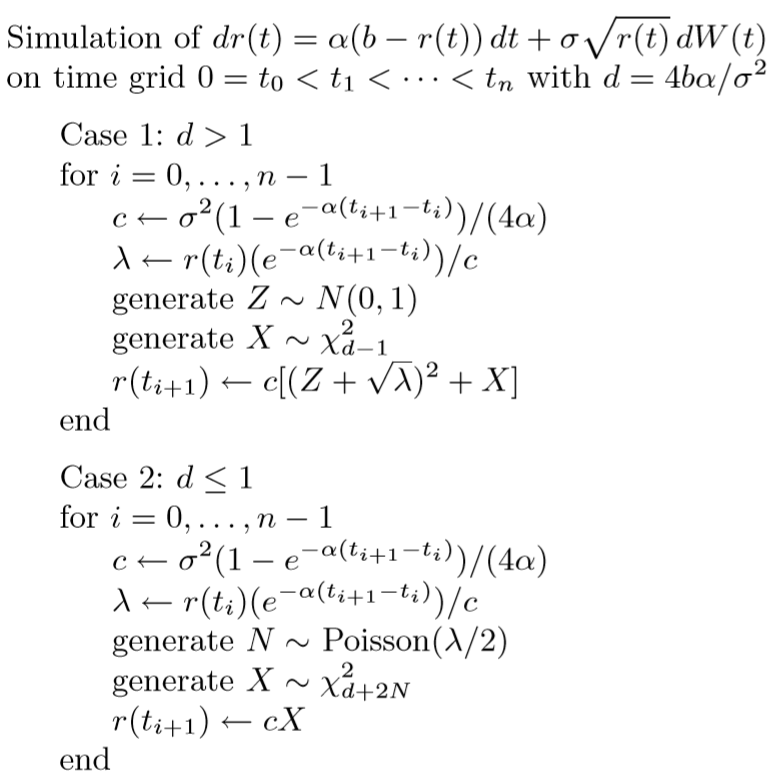
\includegraphics[width=0.75\textwidth]{exact_scheme.png}
\end{frame}

\begin{frame}
\frametitle{Schemes for the CIR process}
\centering
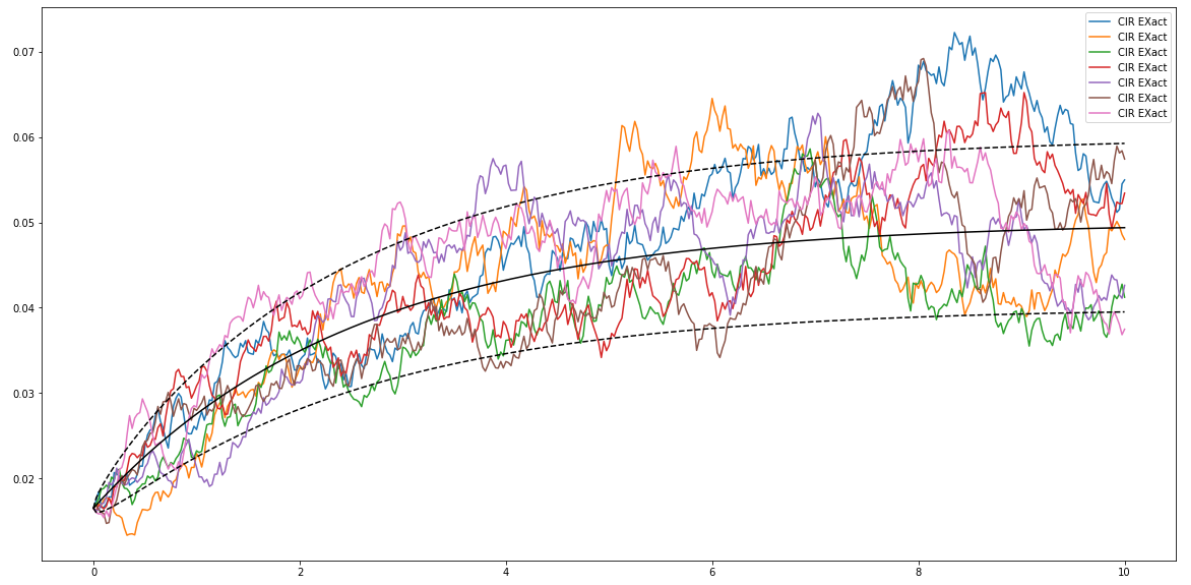
\includegraphics[width=\textwidth]{paths_exact.png}
\end{frame}

\begin{frame}
\frametitle{Schemes for the CIR process}
We can simulate the process exactly provided we can sample from the non chi-square distribution which implies sampling from a Gamma distribution.
\vspace{0.5cm}

$2X \sim \chi_\nu$ where $X \sim gamma(\nu/2,1)$.
\vspace{0.5cm}

Methods for sampling a $gamma(a, 1)$ usually distinguish between $a \leq 1$ and $a > 1$. In our case $a = \frac{2a}{\sigma^2}$.
\vspace{0.5cm}

Exact schemes are drastically too slow if one has to simulate the process along a time-grid which occurs when pricing path-dependent options.

\end{frame}

\begin{frame}
\frametitle{Schemes for the CIR process}
Alternatives:
\vspace{0.5cm}

Euler-Maruyama scheme:

$$ X_{t + 1}^n = X_t^n + \frac{1}{n}(a - kX_t^n) + \frac{\sigma}{\sqrt{n}}\sqrt{X_t^n}Z_t^n$$

Other schemes:

$$ X_{t + 1}^n = X_t^n + \frac{1}{n}(a - kX_t^n) + \frac{\sigma}{\sqrt{n}}\sqrt{(X_t^n)^+}Z_t^n$$

$$ X_{t + 1}^n = |X_t^n + \frac{1}{n}(a - kX_t^n) + \frac{\sigma}{\sqrt{n}}\sqrt{X_t^n}Z_t^n|$$
\end{frame}

\begin{frame}
\frametitle{Second order schemes for the CIR process}
\textbf{\Large{$\sigma^2 \leq 4a$}}
\vspace{0.5cm}

In this case, the \textit{Ninomiya-Victoir} scheme for the CIR process writes:

$$ X_{t + 1}^n = \varphi(X_t^n, \Delta, \sqrt{\Delta}Z)$$

where
\begin{align*}
\varphi(x, t, w) = & e^{-\frac{kt}{2}}(\sqrt{(a - \sigma^2/4)\phi(t/2) +  e^{-\frac{kt}{2}}x} + \frac{\sigma}{2}w)^2 \\
                   & + (a - \sigma^2/4)\phi(t/2)
\end{align*}

\end{frame}

\begin{frame}
	\frametitle{Second order schemes for the CIR process}
	\centering
	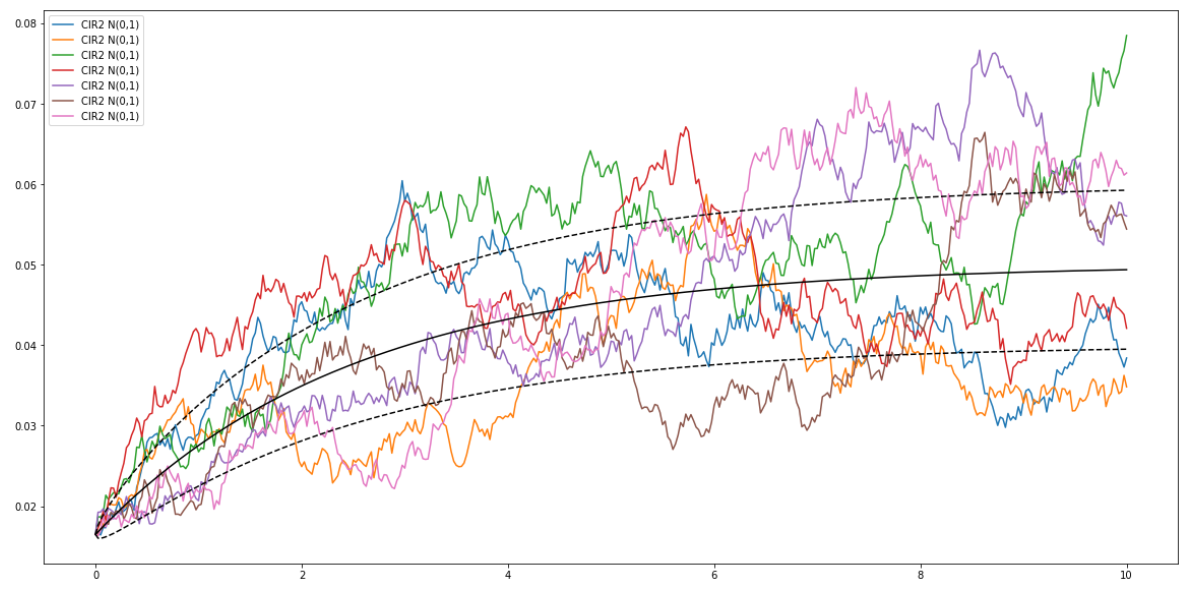
\includegraphics[width=\textwidth]{paths_cir2_N.png}
\end{frame}

\begin{frame}
\frametitle{Second order schemes for the CIR process}
\textbf{\Large{$\sigma^2 > 4a$}}
\vspace{0.5cm}

In this case, the \textit{Alfonsi} scheme for the CIR process writes:

\begin{align*}
	 X_{t + 1}^n =& \varphi(X_t^n, \Delta, \sqrt{\Delta}Y), \hspace{1.5cm} X_t^n \geq 1_{\{\sigma^2 > 4a \}}K_2(\Delta)\\
	 \\
     X_{t + 1}^n =& 1_{\{U \leq \pi(\Delta, X_t^n)\}}A_1(\Delta, X_t^n) + 1_{\{U \ > \pi(\Delta, X_t^n)\}}A_2(\Delta, X_t^n), \\
     \\
                  & \hspace{4.5cm}X_t^n < 1_{\{\sigma^2 > 4a \}}K_2(\Delta)
\end{align*}

Where $Y$ is a discrete bounded variable that fits the five first moments of a standard Gaussian variable.
\end{frame}

\begin{frame}
	\frametitle{Second order schemes for the CIR process}
	\centering
	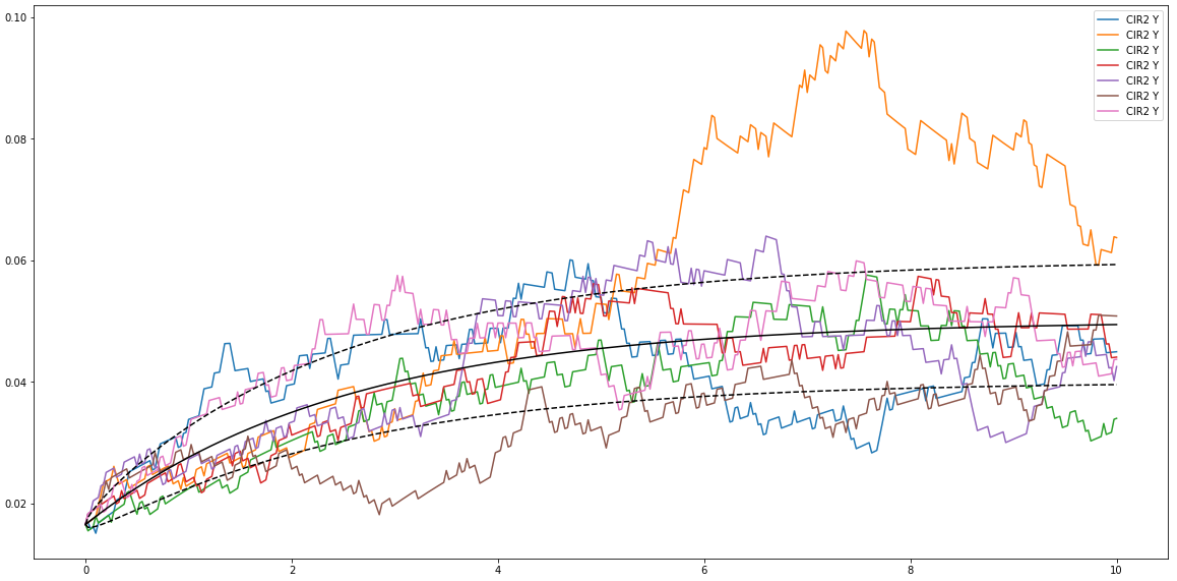
\includegraphics[width=\textwidth]{paths_cir2_Y.png}
\end{frame}

\begin{frame}
	\frametitle{Second order schemes for the CIR process}
	\centering
	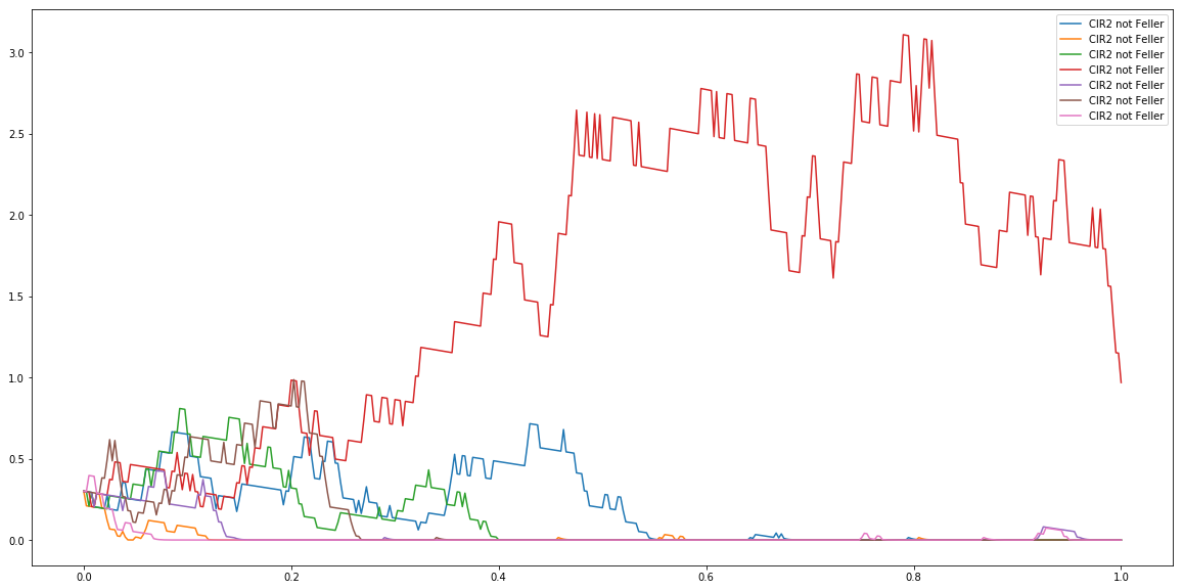
\includegraphics[height=0.4\textheight, width=\textwidth]{paths_cir2_not_feller.png}\\
	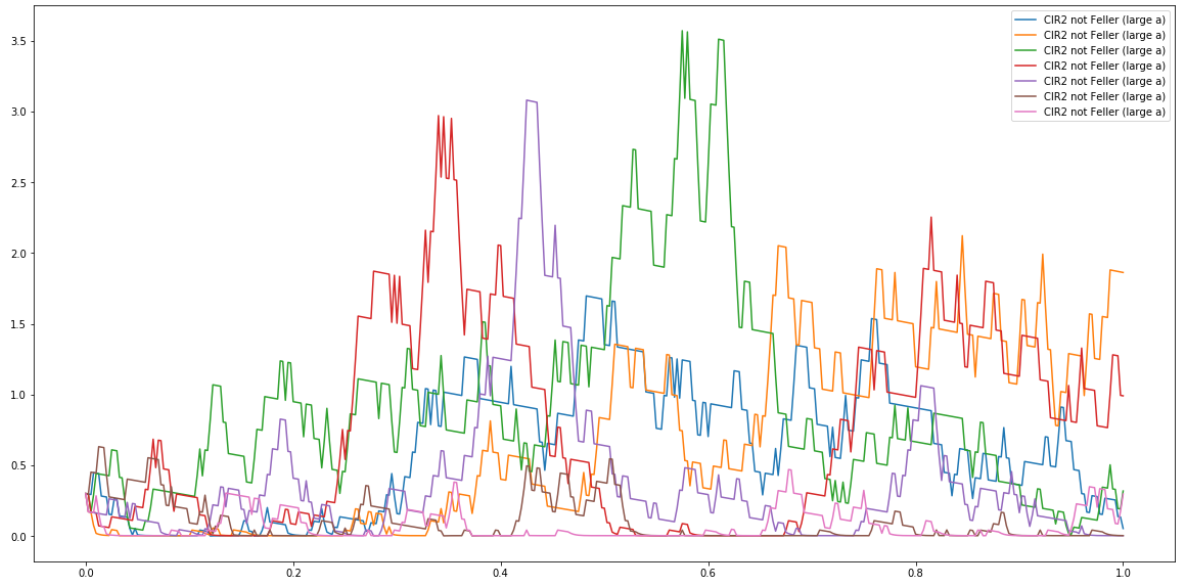
\includegraphics[height=0.4\textheight, width=\textwidth]{paths_cir2_not_feller_large_a.png}
\end{frame}

\begin{frame}
\frametitle{Simulations for the CIR process}
Similarly as in the paper we want to illustrate the convergence of the second order scheme and some of its possible variations.
\vspace{0.1cm}

In order to do this we will compute the quantity $\mathbb{E}[e^{-X_T^n}]$ given by the different schemes and fixing the number of \\paths $= 100000$.
\vspace{0.3cm}

To compute the theoretical value $\mathbb{E}[e^{-X_T}]$ recall that the CIR process has a noncentral chi-square future distribution with $\frac{4a}{\sigma^2}$ degrees of freedom and non-centrality parameter $\frac{4kx_te^{-kt}}{(1 - e^{-kt})\sigma^2}$, so we can use the moment generating function of a chi-square distribution.

\end{frame}

\begin{frame}
	\frametitle{Simulations for the CIR. Feller condition satisfied.}
	\centering
	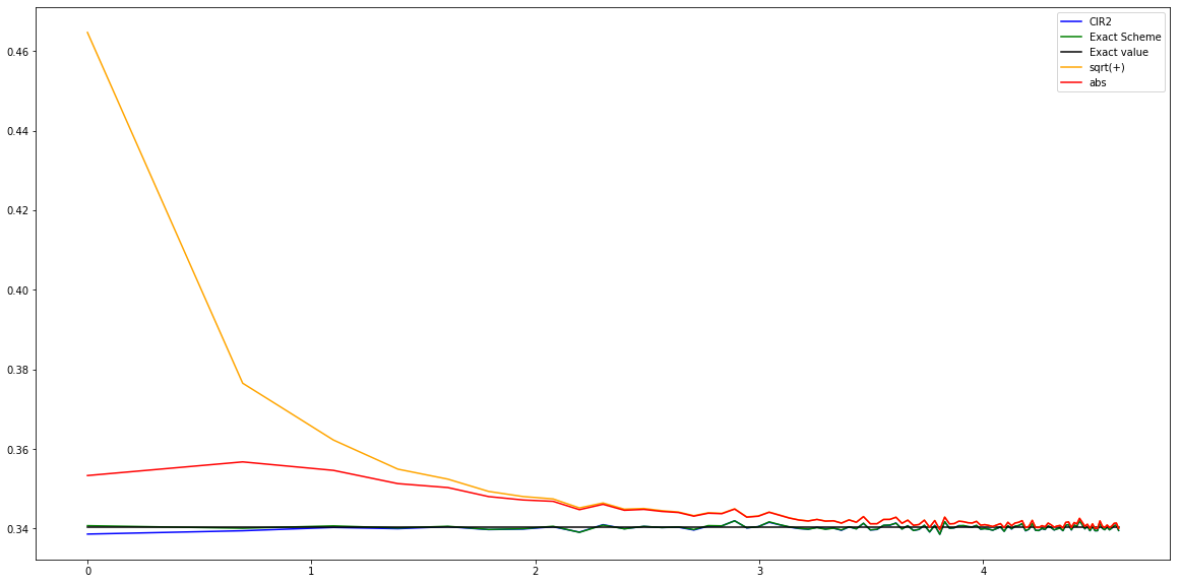
\includegraphics[width=\textwidth]{schemes_feller.png}
\end{frame}

\begin{frame}
	\frametitle{Simulations for the CIR. Feller condition satisfied.}
	\centering
	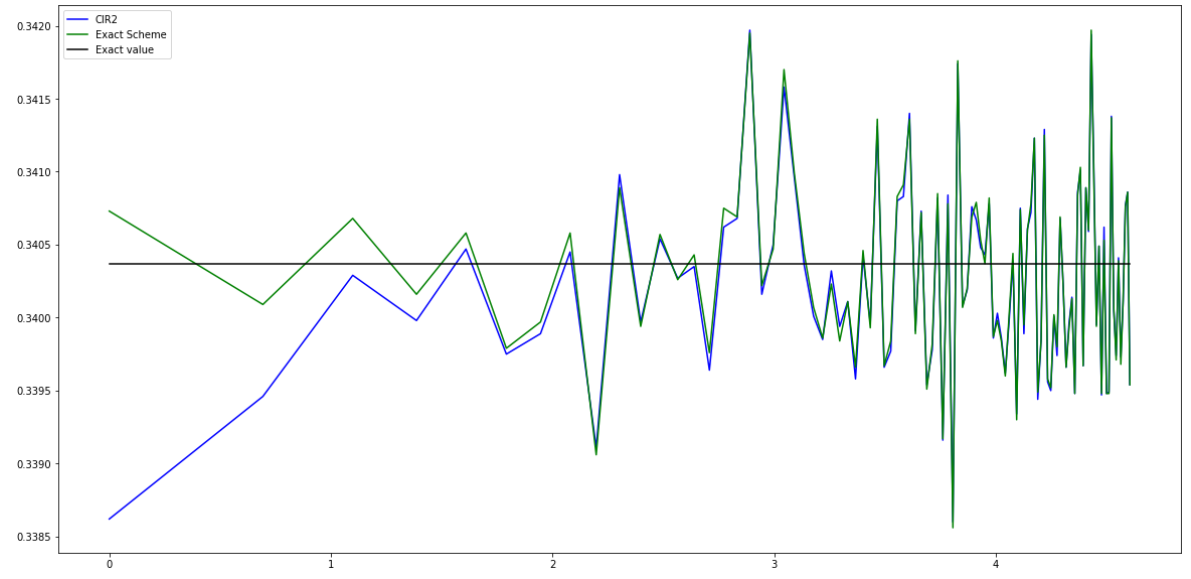
\includegraphics[width=\textwidth]{Exact_CIR2.png}
\end{frame}

\begin{frame}
	\frametitle{Simulations for the CIR. Feller condition satisfied.}
	\centering
	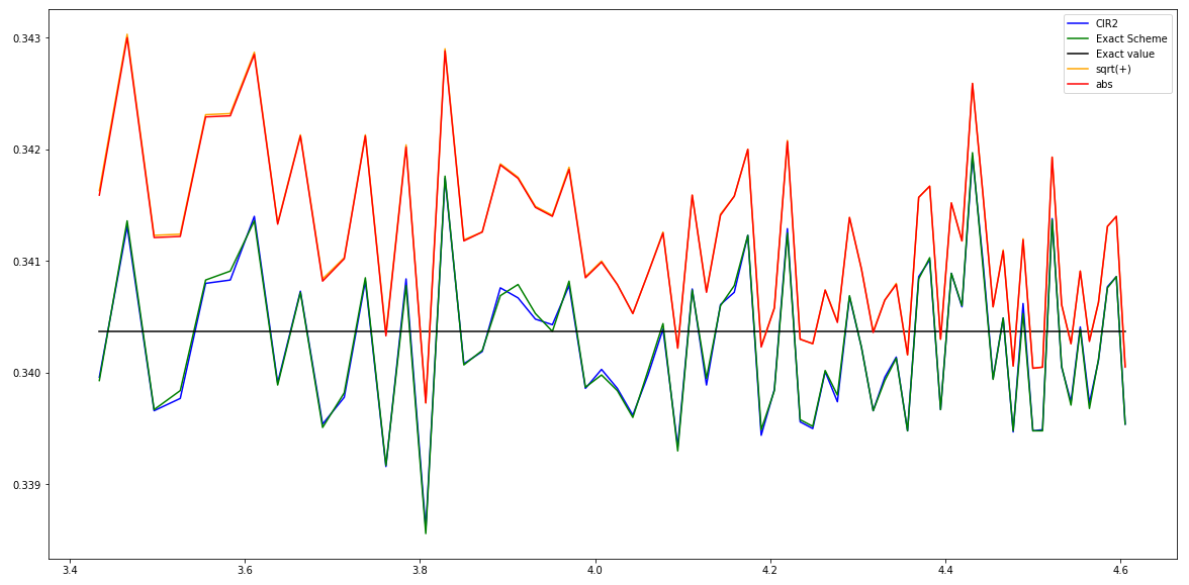
\includegraphics[width=\textwidth]{schemes_feller_30.png}
\end{frame}

\begin{frame}
	\frametitle{Simulations for the CIR. Feller cond. not satisfied.}
	\centering
	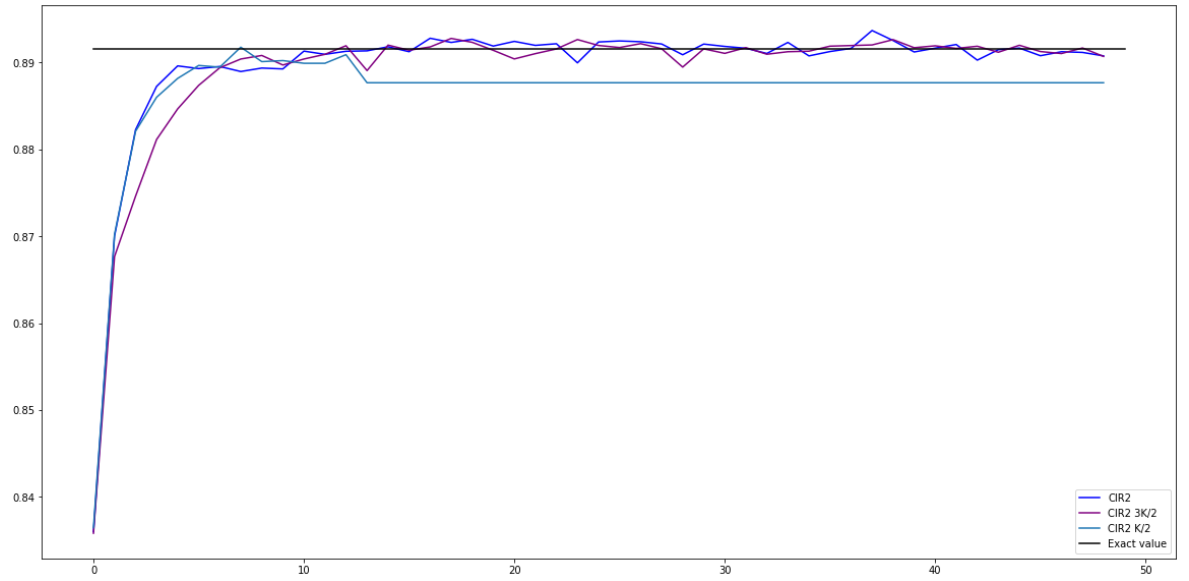
\includegraphics[width=\textwidth]{good_schemes_not_feller.png}
\end{frame}

\begin{frame}
	\frametitle{Simulations for the CIR. Feller cond. not satisfied.}
	\centering
	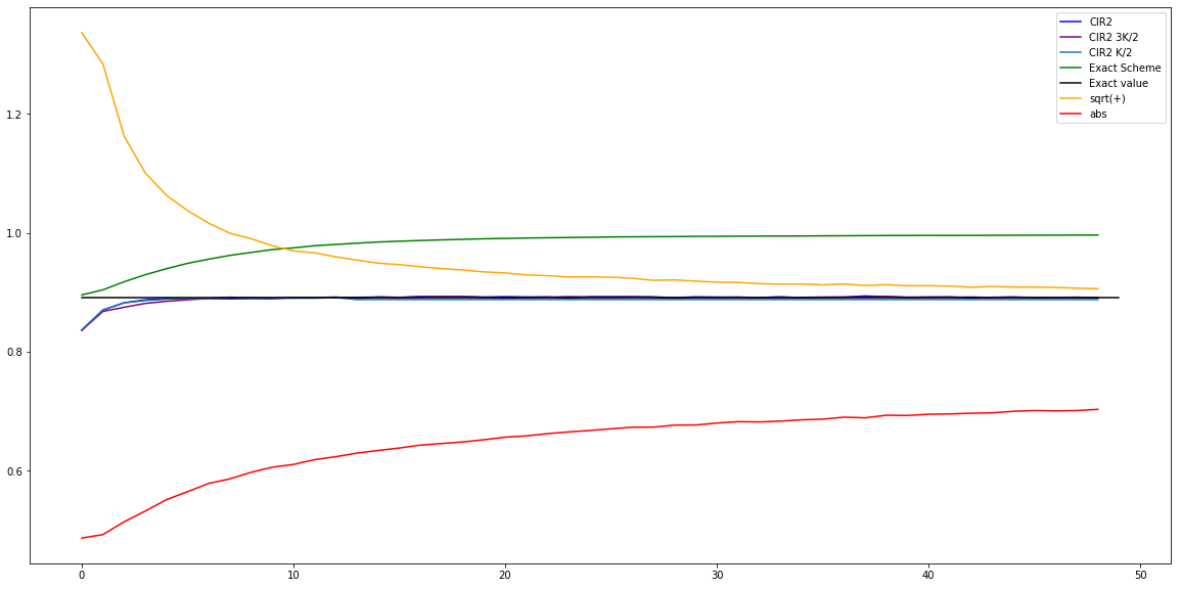
\includegraphics[width=\textwidth]{schemes_not_feller.png}
\end{frame}


\section{Using the Heston Model}
\frame{\tableofcontents[currentsection]}


\begin{frame}
\frametitle{Using the Heston Model - Heston model}
\begin{itemize}
  \item Mathematical model implementing stochastic volatility.
  \item Uses an underlying CIR process for the variance.
\end{itemize}

$$dS_t=\mu S_tdt+\sqrt{\nu_t}S_tdW_t^s$$
$$d\nu_t = \kappa(\theta-\nu_t)dt+\xi\sqrt{\nu_t}dW_t^\nu$$

\end{frame}


\begin{frame}
\frametitle{Using the Heston Model - Calibration}
\begin{itemize}
  \item In order to test the efficiency of the second order scheme, we calibrate the Heston Model using real data. In detail, we use a USDGBP volatility surface which was downloaded in Bloomberg.
  \item To calibrate the Heston model, we use the most liquid option in this market.
\end{itemize}
\end{frame}

\begin{frame}
\frametitle{Using the Heston Model - Calibration}
\centering
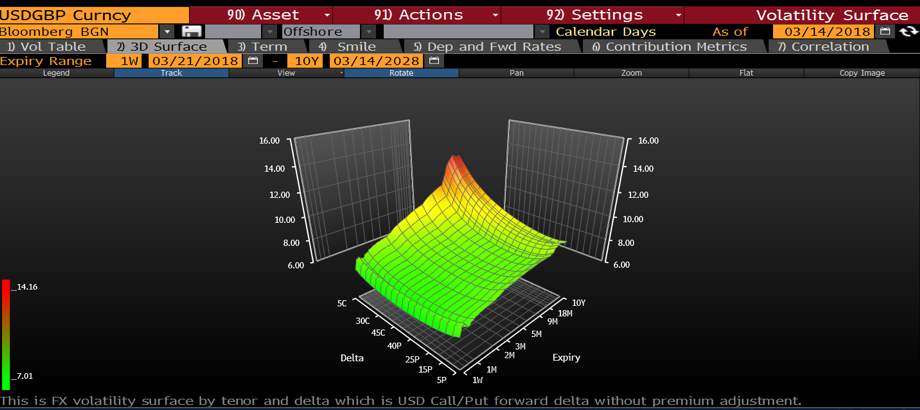
\includegraphics[width=.75\textwidth]{bloomberg1.png}
\\[.5cm]
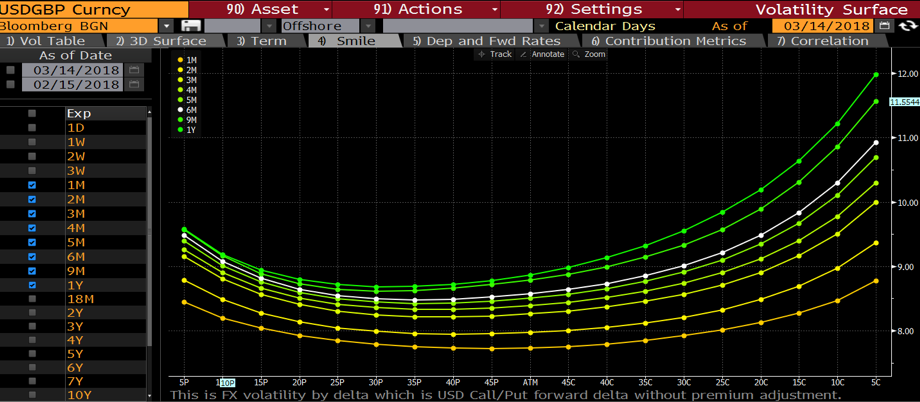
\includegraphics[width=.75\textwidth]{bloomberg2.png}
\end{frame}

\begin{frame}
\frametitle{Using the Heston Model - Calibration}
\begin{itemize}
  \item In the currency option market, prices are quoted for moneyness levels for different time to expiry periods. These moneyness levels are:
  \begin{itemize}
    \item At the money level or at the money forward (50 delta dual),
    \item Out of the money level at 25 delta dual,
    \item In the money level (75 delta dual).
  \end{itemize}
  \item Delta dual is the first derivative with respect to the strike price.
\end{itemize}
$$\Delta_{dual}=\frac{\partial BS_{call}}{\partial k}=e^{-r_{d}}\Phi \left(\frac{ln(S_{0}/K)+(r_{d}-r_{f}-\sigma^{2}(0.5))T}{\sigma \sqrt T}\right)$$
\end{frame}


\begin{frame}
\frametitle{Using the Heston Model - Calibration}
Basically, it is necessary to compute the associated strike for each option in order to compute the following equation:

$$\underset{\theta,\sigma,\rho,\kappa,\eta,\mu}{min}=(BS(\sigma,r,K,S_{0},T)-P_{heston}(\theta,\sigma,\rho,\kappa,\eta,\mu,r,K,S_{0},T))^2$$

When the option is traded in the OTC market, each smile has an associated level of strike. When the option is traded in an exchange market all smiles have the same level of strike.
\end{frame}

\begin{frame}
\frametitle{Using the Heston Model - Calibration}

\begin{align*}
V_0 &= 0.07727 \\
S_0 &= 1.39353 \\
\mu = r &= 0.092 \\
\rho &= -0.7683 \\
\theta &= 0.2572 \\
\sigma &= 0.3484 \\
\kappa &= 1.1159
\end{align*}

\end{frame}

% \begin{frame}
% \frametitle{Using the Heston Model}
% 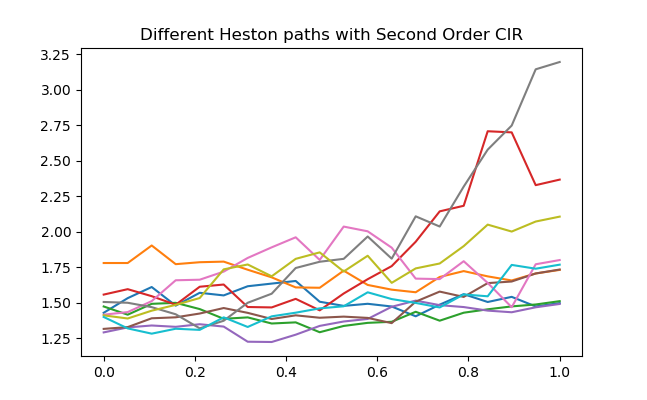
\includegraphics[width=.5\textwidth]{heston_cir220.png}
% 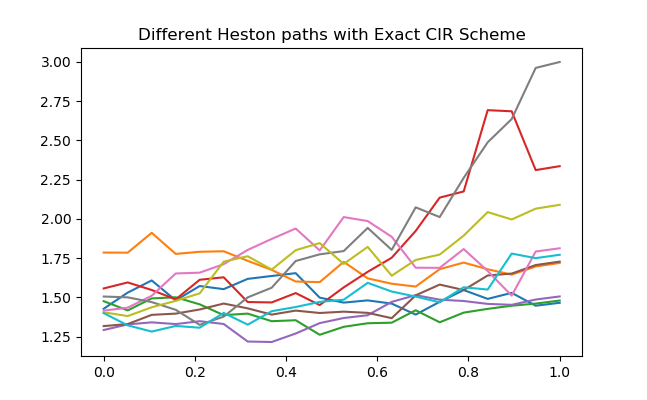
\includegraphics[width=.5\textwidth]{heston_exact20.png}
% \end{frame}

\begin{frame}
\frametitle{Using the Heston Model}
\centering
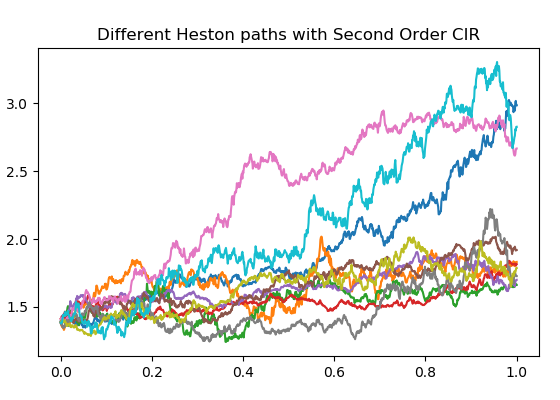
\includegraphics[width=.5\textwidth]{heston_cir21000.png}
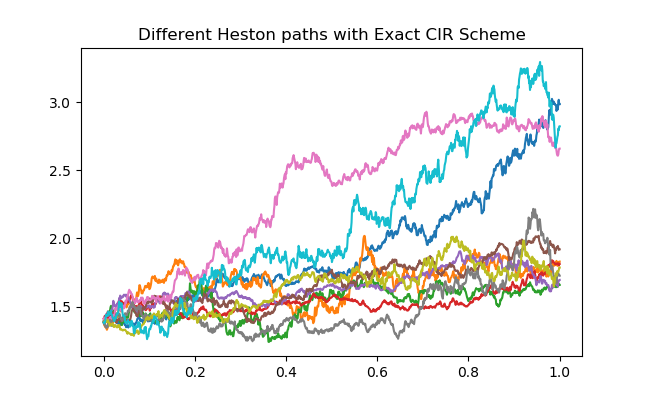
\includegraphics[width=.5\textwidth]{heston_exact1000.png}
\end{frame}

\begin{frame}
\frametitle{Using the Heston Model}
\centering
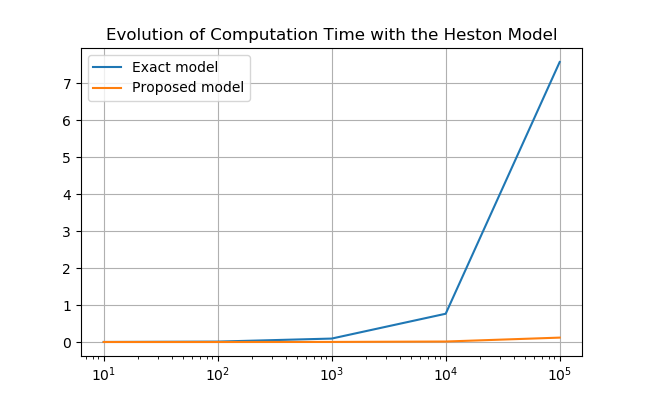
\includegraphics[width=.5\textwidth]{heston_time.png}
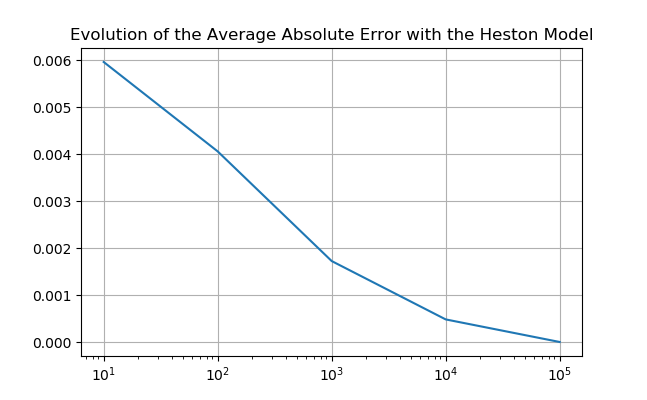
\includegraphics[width=.5\textwidth]{heston_error.png}
\end{frame}

\begin{frame}
\frametitle{Conclusion}
\begin{itemize}
  \item We have succesfully implemented Aurélien Alfonsi's work on CIR second order discretization schemes.
  \item We have tried to calibrate and to simulate the Heston model.
  \item Beyond our work: how would it behave with path-dependent options?
\end{itemize}
\end{frame}


\begin{frame}
\centering
{\Large Thank you!}
\\[1cm]
{\small\url{github.com/tjespel/discretization-cir-processes}}
\end{frame}
\end{document}
